
\begin{minipage}[c]{\textwidth}
\centering
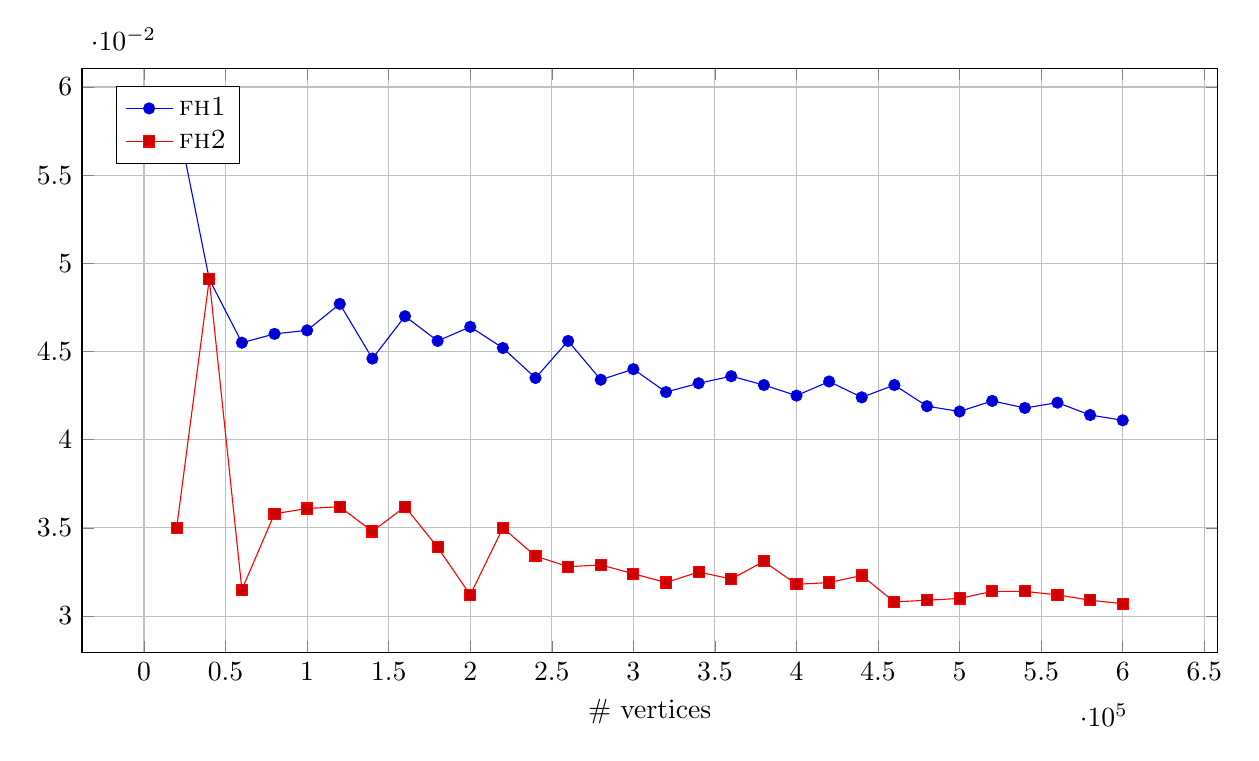
\begin{tikzpicture}
        \begin{axis}[
            xlabel = \# vertices,
            height=9cm,
            width=16cm,
            grid=major,
            legend pos=north west
    	]

        \addplot coordinates {
(20000,0.0583)
(40000,0.0491)
(60000,0.0455)
(80000,0.0460)
(100000,0.0462)
(120000,0.0477)
(140000,0.0446)
(160000,0.0470)
(180000,0.0456)
(200000,0.0464)
(220000,0.0452)
(240000,0.0435)
(260000,0.0456)
(280000,0.0434)
(300000,0.0440)
(320000,0.0427)
(340000,0.0432)
(360000,0.0436)
(380000,0.0431)
(400000,0.0425)
(420000,0.0433)
(440000,0.0424)
(460000,0.0431)
(480000,0.0419)
(500000,0.0416)
(520000,0.0422)
(540000,0.0418)
(560000,0.0421)
(580000,0.0414)
(600000,0.0411)

    	};
        
    	\addlegendentry{\textsc{fh1}}

        \addplot coordinates {
(20000,0.0350)
(40000,0.0491)
(60000,0.0315)
(80000,0.0358)
(100000,0.0361)
(120000,0.0362)
(140000,0.0348)
(160000,0.0362)
(180000,0.0339)
(200000,0.0312)
(220000,0.0350)
(240000,0.0334)
(260000,0.0328)
(280000,0.0329)
(300000,0.0324)
(320000,0.0319)
(340000,0.0325)
(360000,0.0321)
(380000,0.0331)
(400000,0.0318)
(420000,0.0319)
(440000,0.0323)
(460000,0.0308)
(480000,0.0309)
(500000,0.0310)
(520000,0.0314)
(540000,0.0314)
(560000,0.0312)
(580000,0.0309)
(600000,0.0307)

    	};
        
    	\addlegendentry{\textsc{fh2}}


        \end{axis}

    \end{tikzpicture}
    \captionof{figure}{Running time divided by $nlogn$}}
    \label{fig:time_18}
\end{minipage}
